\setcounter{section}{0}
	Độ lớn vận tốc tức thời tại một điểm cho ta biết sự nhanh chậm của chuyển động tại điểm đó:
\begin{equation*}
	v=\dfrac{\Delta s}{\Delta t}.
\end{equation*}	

	Vectơ vận tốc tức thời là một đại lượng vectơ có:
\begin{itemize}
	\item gốc đặt ở vật chuyển động;
	\item hướng là hướng của chuyển động;
	\item độ dài biểu diễn độ lớn của vận tốc.
\end{itemize}

	Gia tốc là đại lượng đặc trưng cho sự biến thiên nhanh hay chậm của vận tốc và được đo bằng thương số giữa độ biến thiên vận tốc $\Delta v$ và khoảng thời gian vận tốc biến thiên $\Delta t$,

\begin{equation*}
	a=\dfrac{\Delta v}{\Delta t}.
\end{equation*}	

	Vì vận tốc là đại lượng vectơ nên gia tốc cũng là đại lượng vectơ:
\begin{equation*}
	\vec{a}=\dfrac{\vec{v}-\vec{v}_0}{t-t_0}=\dfrac{\Delta\vec{v}}{\Delta t}.
\end{equation*}

Vectơ gia tốc tức thời là một đại lượng vectơ có:
\begin{itemize}
	\item gốc đặt ở vật chuyển động;
	\item hướng trùng với hướng vectơ vận tốc nếu chuyển động nhanh dần đều $(a\cdot v > 0)$, ngược hướng vectơ vận tốc nếu chuyển động chậm dần đều $(a\cdot v< 0)$;
	\item độ dài tỉ lệ với độ lớn của gia tốc theo một tỉ xích nào đó.
\end{itemize}

\begin{enumerate}[label=\bfseries Câu \arabic*:]
	\item \mkstar{1}
	
	{
	Hãy chứng tỏ khi $\vec a$ cùng chiều với $\vec v$ ($a\cdot v>0$) thì chuyển động là nhanh dần, khi $\vec a$ ngược chiều với $\vec v$ ($a\cdot v<0$) thì chuyển động là chậm dần.
	}
	\hideall{
		
	+	$a<0$ có nghĩa là chuyển động chậm dần. Mà $a=\dfrac{\Delta v}{\Delta t}$. Trong khi đó $\Delta t$ luôn luôn lớn hơn 0 nên $\Delta v <0 \Leftrightarrow v - v_0 <0 \Leftrightarrow v < v_0$. Suy ra $\vec a$ ngược chiều với $\vec v$.
	
	+  $a>0$ có nghĩa là chuyển động chậm dần. Mà $a=\dfrac{\Delta v}{\Delta t}$. Trong khi đó $\Delta t$ luôn luôn lớn hơn 0 nên $\Delta v >0 \Leftrightarrow v - v_0 ?0 \Leftrightarrow v > v_0$. Suy ra $\vec a$ cùng chiều với $\vec v$.
		
	}
	\item \mkstar{2}
	
	{
	Một ô tô tăng tốc từ lúc đứng yên, sau $\SI{6}{s}$ đạt vận tốc $\SI{18}{m/s}$. Tính độ lớn gia tốc của ô tô.
	}
	\hideall{
		
		Gia tốc của ô tô
		
		$$a = \dfrac{v_2 - v_1}{t} = \dfrac{18 - 0}{6} = \SI{3}{m/s}^2.$$
	}
	\item \mkstar{2}
	
	{
	Người lái xe ô tô hãm phanh để xe giảm tốc độ từ $\SI{23}{m/s}$ đến $\SI{11}{m/s}$ trong $\SI{20}{s}$. Tính độ lớn của gia tốc.
	}
	\hideall{
		
		Độ lớn của gia tốc
		
		$$a = \dfrac{v_2 - v_1}{t} = \dfrac{11-23}{20} = -\SI{0,6}{m/s}^2.$$
	}
		\item \mkstar{2}
	
	{
		Trong một cuộc thi chạy, từ trạng thái đứng yên, một vận động viên chạy với gia tốc $\SI{5}{m/s}^2$ trong 2 giây đầu tiên. Tính vận tốc của vận động viên sau 2 giây.
	}
	\hideall{
		
		Vận tốc của vận động viên
		
		$$a = \dfrac{v_2 - v_1}{t} \Rightarrow v_2 = at = \SI{10}{m/s}.$$
	}
	\item \mkstar{3}
	
	{
		Bảng dưới đây ghi vận tốc tức thời đo bởi tốc kế của một ô tô sau các khoảng thời gian $\SI{2}{s}$ kể từ khi bắt đầu chạy trên một đường thẳng.
		
		\begin{center}
			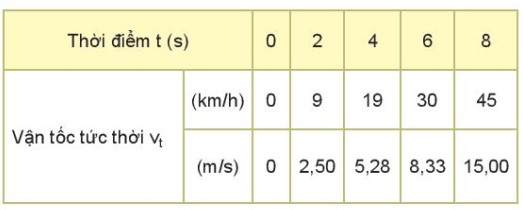
\includegraphics[scale=1]{../figs/VN10-2022-PH-TP007-1.jpg}
		\end{center}
	
		\begin{enumerate}[label=\alph*)]
			\item Xác định độ biến thiên vận tốc sau $\SI{8}{s}$ của chuyển động trên.
			\item Xác định độ biến thiên của vận tốc sau mỗi giây của chuyển động trên trong $\SI{4}{s}$ đầu và trong $\SI{4}{s}$ cuối.
		\end{enumerate}
	}
	\hideall{
		
		\begin{enumerate}[label=\alph*)]
			\item 
			Độ biến thiên vận tốc sau 8 giây là
			
			$$\Delta v = v_8 - v_0 = \SI{45}{km/h}.$$
			\item Độ biến thiên vận tốc trong 4 giây đầu là
			
			$$\Delta v = v_4 - v_0 = \SI{5,28}{m/s}.$$
			
			Độ biến thiên của vận tốc sau mỗi giây của chuyển động trên trong 4 giây đầu là :
			
			$$\dfrac{\Delta v}{\Delta t} = \SI{1,32}{m/s}^.$$
			
			Độ biến thiên vận tốc trong 4 giây sau là: 
			
			$$\Delta v' = v_8 - v_4 =\SI{7,22}{m/s}.$$
			
			Độ biến thiên của vận tốc sau mỗi giây của chuyển động trên trong 4 giây sau là:
			
			$$\dfrac{\Delta v'}{\Delta t} = \SI{1,805}{m/s}^2.$$ 
		\end{enumerate}
	}
		\item \mkstar{3}
	
	{
		Một xe máy đang chuyển động thẳng với vận tốc $\SI{10}{m/s}$ thì tăng tốc. Sau $\SI{5}{s}$ đạt vận tốc $\SI{12}{m/s}.$
		
		\begin{enumerate}[label=\alph*)]
			\item Tính gia tốc của xe.
			\item Nếu sau khi đạt vận tốc $\SI{12}{m/s}$, xe chuyển động chậm dần với gia tốc có độ lớn bằng gia tốc trên thì sau bao lâu xe dừng lại?
		\end{enumerate}
	}
	\hideall{
		
		\begin{enumerate}[label=\alph*)]
			\item Gia tốc của xe
			
			$$a = \dfrac{\Delta v}{\Delta t} = \SI{0,4}{m/s}^2.$$
			
			\item Thời gian xe dừng lại
			
			$$\Delta t' = \dfrac{\Delta v'}{a} = \SI{30}{s}.$$
		\end{enumerate}
		
	}
		\item \mkstar{3}
	
	{
		
		\begin{center}
			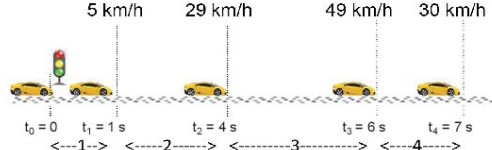
\includegraphics[scale=1]{../figs/VN10-2022-PH-TP007-2.jpg}
		\end{center}
		
		\begin{enumerate}[label=\alph*)]
			\item Tính gia tốc của ô tô trên 4 đoạn đường trên hình.
			\item Gia tốc của ô tô trên đoạn đường 4 có gì đặc biệt so với sự thay đổi vận tốc trên các đoạn đường khác?
		\end{enumerate}
	}
	\hideall{
		
		Ta có:
		
		$v_1 = \SI{5}{km/h}= \SI{1,389}{m/s}.$
		
		$v_2 =\SI{29}{km/h}= \SI{8,056}{m/s}.$
		
		$v_3 = \SI{49}{km/h}= \SI{13,61}{m/s}.$
		
		$v_4 = \SI{30}{km/h}= \SI{8,33}{m/s}.$
		\begin{enumerate}[label=\alph*)]
			\item Gia tốc của ô tô trên 4 đoạn đường
			
			$$a_1 = \dfrac{v_1 - 0}{t_1 - t_0} = \SI{1,389}{m/s}^2.$$
			
			$$a_2 = \dfrac{v_2 - v_1}{t_2 - t_1} = \SI{2,222}{m/s}^2.$$
			
			$$a_3 = \dfrac{v_3 - v_2}{t_3 - t_2} = \SI{2,777}{m/s}^2.$$
			
			$$a_4 = \dfrac{v_4 - v_3}{t_4 - t_3} = - \SI{5,28}{m/s}^2.$$
			
			\item Gia tốc trên đoạn đường 4 mang dấu âm (-) khác hơn so với gia tốc trên 3 đoạn đường còn lại. Điều này là do ô tô chạy chậm lại.
		\end{enumerate}
	}
		\item \mkstar{3}
	
	{
		
		Một con báo đang chạy với vận tốc $\SI{30}{m/s}$ thì chuyển động chậm dần khi tới gần một con suối. Trong 3 giây, vận tốc của nó giảm còn $\SI{9}{m/s}$. Tính gia tốc của con báo.
	}
	\hideall{
		
		Gia tốc của con báo là:
		
		$$a = \dfrac{v_2 - v_1}{t} = - \SI{9}{m/s}^2.$$
	}
		\item \mkstar{3}
	
	{
		
	Đồ thị mô tả sự thay đổi vận tốc theo thời gian trong chuyển động của một ô tô thể thao đang chạy thử về phía Bắc. Tính gia tốc của ô tô:
	\begin{center}
		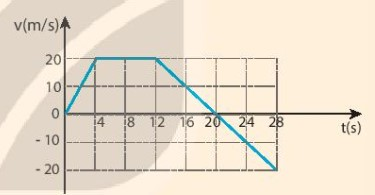
\includegraphics[scale=1]{../figs/VN10-2022-PH-TP007-3.jpg}
	\end{center}
	
	\begin{enumerate}[label=\alph*)]
		\item Trong $\SI{4}{s}$.
		\item Từ giây thứ 4 đến giây thứ 12.
	\end{enumerate}
	}
	\hideall{
		
		\begin{enumerate}[label=\alph*)]
			\item Trong $\SI{4}{s}$
			
			$$a_1 = \dfrac{20 -0}{4- 0} = \SI{5}{m/s}^2.$$
			
			\item Từ giây thứ 4 đến giây thứ 12
			
			$$a_2 = \dfrac{20 - 20}{12-4} = \SI{0}{m/s}^2.$$
			
			
		\end{enumerate}
	}
		\item \mkstar{3}
	
	{
		
		Đồ thị mô tả sự thay đổi vận tốc theo thời gian trong chuyển động của một ô tô thể thao đang chạy thử về phía Bắc. Tính gia tốc của ô tô:
		\begin{center}
			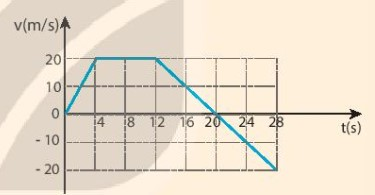
\includegraphics[scale=1]{../figs/VN10-2022-PH-TP007-3.jpg}
		\end{center}
		
		\begin{enumerate}[label=\alph*)]
			\item Từ giây thứ 12 đến giây thứ 20.
			\item Từ giây thứ 20 đến giây thứ 28.
		\end{enumerate}
	}
	\hideall{
		
		\begin{enumerate}[label=\alph*)]
			\item Từ giây thứ 12 đến giây thứ 20
			
			$$a_3 = \dfrac{0 - 20}{20-12} = -\SI{2,5}{m/s}^2.$$
			
			\item Từ giây thứ 20 đến giây thứ 28
			
			$$a_4 = \dfrac{-20 - 0}{28 -20} = -\SI{2,5}{m/s}^2.$$
		\end{enumerate}
	}
\end{enumerate}